% This is LLNCS.DEM the demonstration file of
% the LaTeX macro package from Springer-Verlag
% for Lecture Notes in Computer Science,
% version 2.4 for LaTeX2e as of 16. April 2010
%
\documentclass{llncs}
%
\usepackage{amsfonts}
\usepackage{comment}
\usepackage{graphicx}
\usepackage{caption}
\usepackage{subcaption}
\usepackage{verbatim}
\usepackage{url}

\newcommand{\SunroofAnalog}[1]{#1\ensuremath{_\downarrow}}
\newcommand{\HaskellAnalog}[1]{#1\ensuremath{_\uparrow}}

%\newcommand{\NOTE}[1]{{\Large\textbf{NOTE:}\ #1}}
\newcommand{\TODO}[1]{{(\textbf{TODO:}\ #1)}}
\newcommand{\Src}[1]{{\tt{#1}}}

\newcommand{\IO}{\Src{IO}}
\newcommand{\JS}{\Src{JS}}
\newcommand{\JSI}{\Src{JSI}}
\newcommand{\JSA}{\ensuremath{\Src{JS}_\Src{A}}}
\newcommand{\JSB}{\ensuremath{\Src{JS}_\Src{B}}}

\newcommand{\Figure}[3]{%
\FigureS{#1}{#2}{#3}{scale=0.55,clip=true,trim=0.45cm 0.45cm 0.45cm 0.45cm}
}

\newcommand{\FigureS}[4]{%
\begin{figure}[t]%
%\vspace{-0.5cm}%
\begin{center}%
\includegraphics[#4]{#2}%
\vspace{-0.5cm}%
\end{center}%
\caption{#3}%
\label{#1}%
\end{figure}%
}

\newenvironment{Code}{\verbatim}{\endverbatim}

\newcommand{\FigRef}[1]{Fig.~\ref{#1}}
\newcommand{\SecRef}[1]{Section~\ref{#1}}
\newcommand{\TabRef}[1]{Table~\ref{#1}}

% intentional for the referee's copy
\pagestyle{plain}
\newcommand{\CURSOR}{\noindent\rule{\textwidth}{4pt}}

\begin{document}
%
\title{Sunroof: A Monadic DSL for Generating JavaScript}
%\subtitle{}
%
\titlerunning{Sunroof}  % abbreviated title (for running head)
%                                     also used for the TOC unless
%                                     \toctitle is used
%
\author{Andy Gill\inst{1} and Jan Bracker\inst{1,2}}
%
\authorrunning{Jan Bracker \and Andy Gill} % abbreviated author list (for running head)
%
%%%% list of authors for the TOC (use if author list has to be modified)
\tocauthor{Andy Gill, Jan Bracker}
%
\institute{%
ITTC / EECS \\
The University of Kansas, Lawrence, KS 66045\\
~\\
\and
Institut f{\"u}r Informatik\\
Christian-Albrechts-Universit{\"a}t, Kiel, Germany}

\maketitle

\begin{abstract}        
Sunroof is a Haskell-hosted Domain Specific Language (DSL) for generating JavaScript.
Sunroof is built on top of the JavaScript monad, which, like the Haskell \IO-monad, allows 
access to external resources, but specifically JavaScript
resources. As such, Sunroof is primarily a feature-rich 
foreign-function API to the browser's JavaScript engine, and all the browser-specific
functionality, including HTML-based rendering, event handling, and 
drawing to the HTML5 canvas. 

In this paper, we give the design and implementation of Sunroof.
Using monadic reification, we generate JavaScript from
a deep embedding of the JavaScript monad.
The Sunroof DSL has the feel of native Haskell, with a simple
Haskell-based type schema to guide the Sunroof programmer.
Furthermore, because we are generating code,
we can offer Haskell-style concurrency patterns, such as MVars and Channels.
In combination with a web-services package,
the Sunroof compiler offers a robust platform to build interactive web applications.

\keywords{DSLs, JavaScript, Web Technologies, Cloud Computing}
\end{abstract}
%
%%%%%%%%%%%%%%%%%%%%%%%%%%%%%%%%%%%%%%%%%%%%%%%%%%%%%%%%%%%%%%%%%%%%%%%%%%%%%%%%%%%%%%%%%%%%%%%%
%%%%%%%%%%%%%%%%%%%%%%%%%%%%%%%%%%%%%%%%%%%%%%%%%%%%%%%%%%%%%%%%%%%%%%%%%%%%%%%%%%%%%%%%%%%%%%%%
%%%%%%%%%%%%%%%%%%%%%%%%%%%%%%%%%%%%%%%%%%%%%%%%%%%%%%%%%%%%%%%%%%%%%%%%%%%%%%%%%%%%%%%%%%%%%%%%

\section{Introduction}\label{sec:intro}

% Simon: Describe the problem
There are many reasons to want to program in a functional language:
efficiency of development cost, informally reasoning, high-level 
control- and concurrency-structures, like monads~\cite{...}.
However, mainstream languages often have better environmental support
than what is provided by functional languages,
for example the Objective C and the iOS ecostructure, or JavaScript and HTML5
web browsers.
This paper examines the challenges of providing
an intentionally blurred interface between Haskell
and JavaScript, to support the development of web-based applications.

% Simon: State your contributions
JavaScript is an imperative language with access to a wide range
of established and useful services like graphical canvases and event
handling of browser events. 
We want to express JavaScript in Haskell, adding use
of Haskell's static typing, and gaining access to JavaScript services
in the browser directly in Haskell.


One way of providing access to non-native services,
such as the JavaScript HTML5 canvas, is to provide, in Haskell, 
foreign function ``hooks'' to key JavaScript functionality,
and compile Haskell to JavaScript by rewriting the
compiler backend.
Haskell already provides many similar hooks into the C RTS,
so why not into a JavaScript?
There are already a number of systems attempting this~\cite{...}.
If executed well, this would be ideal,
but there are engineering shortcomings: 
many standard libraries and hackage packages are not supported directly,
the generated code is not as efficiently executed as native Haskell,
the runtime system is often incomplete. These compilers will continue
to improve, and with initiatives like asm.js~\cite{...},
the efficiency gap many be possible to close.

Rather than rewrite the compiler and runtime system,
an alternative approach is to keep the existing
runtime system, and provide the same 
foreign function ``hooks'' to key JavaScript functionality,
but instead the executed Haskell becomes a server that JavaScript,
and the browser, interact with.
Unfortunately, every JavaScript call becomes an expensive proposition: an RPC call
to a browser.
Though some straight-line calls can be batched together --
our own blank-canvas hackage package~\cite{Hackage:11:blank-canvas} was built on this idea --
the granularity of interaction through JavaScript call is just too fine for
this idea to scale well.

Another approach, and the one we investigate,
is to use a deeply embedded Domain Specific Language (DSL), and
monad reification~\cite{..,..}.
A Haskell-hosted deeply embedded DSL is where Haskell combinators 
are used to build syntactical forms in the target language,
in this case JavaScript.
Monad reification is where binding in a monad can be represented
in a way that they can be captured, and translated into bindings
in a target language.
Historically, these embeddings have worked well for 
data-flow, for example generating combinatorial hardware,
but had serious challenges with capturing binding and control flow.
The mismatch between bindings in the native language (Haskell) 
and the non-native generated code (JavaScript variable names),
reflected through to the usage of the DSL.

This paper uses the recently discovered capability to have monadic-binding
in the DSL to be translated into
bindings in a target language, and then scaling the DSL to support larger examples.
With binding done using regular Haskell monadic binding, 
the language fits naturally with what we would expect from a monadic API. 
In a previous paper, we showed, using a prototype,
that reification of a JavaScript-like language is possible~\cite{Farmer:12:WebDSLs}.
In this paper, we expand on this observation,
and show that monadic-reification is useful in practice.

Building on this DSL, we also investigate providing
JavaScript control flow and function abstraction mechanisms
to the Haskell programmer interested in using the browser API.
Though for technical reasons we can not directly compile
pattern matching and let-binding to JavaScript without committing
to a full Haskell to JavaScript compiler, both
control flow and function abstraction can be provided
with a small syntactical overhead, and reifiable fix-points 
with a modest syntactical overhead.
With these capabilities, a programmer can start programming
using the provided JavaScript API directly, and refine
their program to migrate more and more computation
from the server into the browser. 

%%%%%%%%%%%%%%%%%%%%%%%%%%%%%%%%%%%%%%%%%%%%%%%%%%%%%%%%%%%%%%%%%%%%%%%%%%%%%%%%%%%%%%%%%%%%%%%%
%%%%%%%%%%%%%%%%%%%%%%%%%%%%%%%%%%%%%%%%%%%%%%%%%%%%%%%%%%%%%%%%%%%%%%%%%%%%%%%%%%%%%%%%%%%%%%%%
%%%%%%%%%%%%%%%%%%%%%%%%%%%%%%%%%%%%%%%%%%%%%%%%%%%%%%%%%%%%%%%%%%%%%%%%%%%%%%%%%%%%%%%%%%%%%%%%

\section{Calling JavaScript from Haskell}
\label{sec:js-rpc}

From a programmers' point of view, calling JavaScript functions
appears straightforward. We, as a community know how to reflect an
API into Haskell, using the IO monad. Furthermore, objects in
the target API become handles in Haskell. 

As a first example, consider this simplified example of Sunroof code, and corresponding JavaScript.
\noindent
\begin{Code}
-- Haskell                          // JavaScript
ioCode :: IO ()
ioCode = send jsCode

jsCode :: JS ()
jsCode = do                        function jsCode() {
   name <- prompt "Your name?"       var v0 = prompt("Your name?"); 
   alert ("Your name: " <> name)     alert("Your name: " + v0); 
                                   }
\end{Code}%     
%\noindent 

Here, we use a new monad, the \Src{JS} monad, our JavaScript
analog to the \Src{IO} monad,
and an explicit \Src{send} command that sends the JavaScript to the browser.
This reversal of control, where the
server sends the clients commands is called the Ajax Comet~\cite{..},
or simply long polling.
This interface also bundles the \Src{prompt} and \Src{alert} commands
into one interaction transaction.
It is this flavor of interface we want to support in our Sunroof compiler
and web server.  

To make Sunroof a viable interface to JavaScript, we need to
resolve the following issues:
\begin{itemize}
\item JavaScript is an object-based, imperative, dynamically typed language.
Haskell is a pure, function-based, statically typed language.
In section~\ref{sec:object-model}, we introduce expressions and statements
in Sunroof, and how they jointly form an object model,
mapping these two worlds map together.
%
\item We need to select a concurrent model for Sunroof.
JavaScript natively only supports non-blocking threads.
In section~\ref{sec:threading-models}, we give the
Sunroof interface for providing both non-blocking and blocking cooperative threads,
using the type system to delimit the two concurrency models.
%
\item We choose to provide a way of defining functions
in Sunroof such that they are first-class functions
in JavaScript. In section~\ref{sec:functions-continuations},
we show how we support both functions and continuations.
%
\item We need to provide a foreign function interface,
to allow us to call specific JavaScript-native functions,
like \Src{prompt} and \Src{alert}.
In section~\ref{sec:ffi} we present this interface.
%
\item Critically, we need to be able to compile our Sunroof DSL
into JavaScript. We examine this in section~\ref{sec:compiler}.
\item To enable the compiled code to dynamically interact with
a web browser, we provide an expansion of the \Src{send} idea above,
which we discuss in section~\ref{sec:server}.
\end{itemize}

We close with a small case study, related work, and our conclusions.

%%%%%%%%%%%%%%%%%%%%%%%%%%%%%%%%%%%%%%%%%%%%%%%%%%%%%%%%%%%%%%%%%%%%%%%%%%%%%%%%%%%%%%%%%%%%%%%%
%%%%%%%%%%%%%%%%%%%%%%%%%%%%%%%%%%%%%%%%%%%%%%%%%%%%%%%%%%%%%%%%%%%%%%%%%%%%%%%%%%%%%%%%%%%%%%%%
%%%%%%%%%%%%%%%%%%%%%%%%%%%%%%%%%%%%%%%%%%%%%%%%%%%%%%%%%%%%%%%%%%%%%%%%%%%%%%%%%%%%%%%%%%%%%%%%


\section{Sunroof Values}
\label{sec:object-model}

In the Sunroof DSL, like Haskell itself, we make a distinction between expressions and statements.

\subsection{Sunroof Expressions}

In JavaScript, there are a small number of core types, such as \Src{object}, \Src{array}, and \Src{string}.
In our JavaScript object model, there is a reflection of this family of core types, all prefixed with \Src{JS}.
There is support for booleans, strings, numbers, functions,
object and arrays, and other common programming structures.
The use of \Src{JSNumber}, rather than (say) \Src{Double},
explicitly reminds us of the enforced diminished capabilities of
being within an embedded language,
and all of the \Src{JS}-types are representable in our target language.
Table~\ref{tab:sunroof-types} enumerates major \Src{JS} types used in Sunroof.

\begin{table}[t]
\begin{center}
\begin{tabular}{r@{\quad}l@{\quad}l@{\quad}c}
\hline\rule{0pt}{12pt}%
  Constraint
  & Sunroof Type $\tau$
  & Haskell Analog \HaskellAnalog{$\tau$}
  & \Src{js} \\ \hline\rule{0pt}{12pt}%
  
  & \Src{()}       & \Src{()}     & $\checkmark$ \\
  & \Src{JSBool}   & \Src{Bool}   & $\checkmark$ \\
  & \Src{JSNumber} & \Src{Double} & $\checkmark$ \\
  & \Src{JSString} & \Src{String} & $\checkmark$ \\
  
  \Src{Sunroof $\alpha$}
  & \Src{JSArray $\alpha$} 
  & \Src{[$\HaskellAnalog{\alpha}$]}
  & \\
  
  \Src{SunroofKey $\alpha$}
  & \Src{JSMap $\alpha$ $\beta$}
  & \Src{Map $\HaskellAnalog{\alpha}$ $\HaskellAnalog{\beta}$}
  & \\
  \Src{Sunroof $\beta$} \\
  
  \Src{SunroofArgument $\alpha$}
  & \Src{JSFunction $\alpha$ $\beta$ }
  & \Src{$\HaskellAnalog{\alpha}$ $\rightarrow$ JS$_\Src{A}$ $\HaskellAnalog{\beta}$} 
  & \\
  \Src{Sunroof $\beta$} \\

  \Src{SunroofArgument $\alpha$}
  & \Src{JSContinuation $\alpha$}
  & \Src{$\HaskellAnalog{\alpha}$ $\rightarrow$ JS$_\Src{B}$ $\beta$} 
  & \\
  
  \Src{SunroofArgument $\alpha$}
  & \Src{JSMVar $\alpha$}
  & \Src{MVar $\HaskellAnalog{\alpha}$}
  & \\
  
  \Src{SunroofArgument $\alpha$}
  & \Src{JSChan $\alpha$}
  & \Src{Chan $\HaskellAnalog{\alpha}$}
  & \\[2pt]
\hline
\end{tabular}
\end{center}
\caption{Sunroof types and their Haskell analogs.}
\label{tab:sunroof-types}
\end{table} 

The left-hand column of table~\ref{tab:sunroof-types} gives constraints,
implemented via Haskell type classes.
\begin{itemize}
\item  All our core types are brought together with the \Src{Sunroof} class.
If a type is an instance of \Src{Sunroof}, then that type can be realized inside JavaScript.
All the \Src{JS} types are instances of \Src{Sunroof}.

\item Instances of the \Src{SunroofArgument} class
are values that can be passed to JavaScript functions and methods,
including tuples of values which are used for representing multi-argument 
function calls.
The asymmetry here is a reflection of the JavaScript
asymmetry inherited from C: you can pass multiple arguments
to a function, but only get a single thing back.

\item Finally, there is a third class, \Src{SunroofKey}, which is
is a JavaScript version of the Haskell \Src{Show} class,
but specifically for generating JavaScript object keys.
which are realized as JavaScript strings.
\end{itemize}

Using our \Src{JS}-types, we can build expressions using the traditional Haskell expression-build
mechanisms. \Src{JSNumber} is overloaded, and thus can be used directly for arithmetic.
\Src{JSBool} is an instance of the relevant classes in the hackage package \verb|boolean|.
Further, \Src{JSString} is a \Src{Monoid}~\cite{..}, which is only possible because JavaScript
strings are immutable values.

To help the conversion between classical Haskell values and Sunroof values,
we provide the overloaded function \Src{js}. The right-hand column of 
table~\ref{tab:sunroof-types} shows what types can be converted on the fly.
Putting the expression-building capability together, 
along with a show function called \Src{string}, we can write:
\begin{Code}
alert ("n =  " <> js (n :: Int) <> " n " <> string (m :: JSNumber))
\end{Code}
Here, \Src{n} is a Haskell \Src{Int}, and \Src{m} is a Sunroof number,
presumably the result of a previous computation. Given that we are 
bundling expressions to send to a browser for execution, \Src{n}
is a static value, and \Src{m} is a dynamic value, unobservable until inside our browser's execution.

One design decision in Sunroof is that we enforce a stronger typing than JavaScript itself would.
Specifically, there are restrictions on the type arguments of our container types,
like \Src{JSArray}. What can be seen from this is that we
enforce a Hindley–Milner style thinking to our containers,
which is distinct from JavaScript dynamic typing.
Some types involve
phantom types to give imposed type safety \cite{Cheney:03:FirstClassPhantomTypes}.
Thus, \Src{JSArray} is a restricted type of JavaScript \Src{array}, that, like Haskell,
only support collections of the same type.

From experience with using Sunroof,
the mis-match in typing between Haskell and Sunroof/JavaScript
is not large problem in practice.
However, sometime casting between types, which is implicit in JavaScript,
is needed. So we provide an explicit dynamic \Src{cast},
for use where the type-systems differ,
and both sides of the \Src{cast} are instances of \Src{Sunroof}.
\begin{Code}
cast :: (Sunroof a, Sunroof b) => a -> b
\end{Code}

\subsection{Sunroof Statements}

The building block of object-oriented programing is calling an object's method.
This is almost universally done using the dot (\Src{.}) operator. JavaScript, or target language, 
follows this trend, with the method-call syntax being as follows:
\begin{Code}
  // JavaScript
  object.method(a1,a2,a3,...,aN)
\end{Code}
For our Sunroof object model, we want to model this as close as possible.
We, by convention, have our method calls take the object as the {\em last\/} argument,
and use a monad, called the \Src{JS} monad, for the result because method calls are effectful.
\begin{Code}
// Shape of a Sunroof method
(SunroofArgument args, Sunroof res) => args -> (JSObject -> JS res)
\end{Code}
A neat way of writing method calls in Haskell is transcribing the JavaScript dot, which is already use
for both namespace resolution and function composition in Haskell, with the \Src{\#} combinator~\cite{Shields:01:Babel}.
The \Src{\#} combinator simply applies the second argument to the first (object) argument.
\begin{Code}
// Sunroof        
(#) :: a -> (a -> JS b) -> JS b
(#) obj act = act obj
\end{Code}

\noindent
This gives the follow fragment for a Sunroof call to \Src{method} on \Src{object}.
\begin{Code}
  object # method (a1,a2,a3,...,aN)
\end{Code}
In this way, JavaScript can be transliterated into Haskell where needed,
native JavaScript call idioms can be used,
while other Haskell abstraction mechanisms can be used for the interface that calls Sunroof code.

We piece together our Sunroof method calls using the Haskell support for monads.
\begin{Code}
  r1 <- object # method1 (a1,a2,a3,...,aN)
  r2 <- object # method2 (... can use r1 ...)
  ....
\end{Code} 
In this fragment, \Src{r1} is bound to the result of the \Src{method1} call,
and can be used as an argument to \Src{method2}.

Sometimes, a JavaScript API requires direct access to object attributes.
We do so using a typed \Src{JSSelector}.
\begin{Code}
label :: JSString -> JSSelector a
(!)   :: (Sunroof o, Sunroof a) => o -> JSSelector a -> a
(:=)  :: (Sunroof a, Sunroof o) 
      => JSSelector a -> a -> (o -> JS t ())
\end{Code}
We can build a selector (\Src{label}), use a selector to access a attribute in a specific
object (\Src{!}), or update an attribute in a specific object (\Src{:=}).
The update is in our object-normal-form, that is the object is the final argument.
Sunroof is, in essence, a strict functional language, with monads for effect.
We choose to support direct (non-monadic) reading of attributes, but
all updating of objects requires the monad.
This is a design decision we may return to in the future.

The net effect is that assignments to fields can be neatly expressed,
with a syntax close to JavaScript itself. Our HTML5 canvas library,
build on top of Sunroof primitives, allows the following transliteration
from textbook JavaScript into Sunroof:

\begin{Code}
  // JavaScript                         // Sunroof
  c.fillStyle = "red";                  c # fillStyle := "red"
\end{Code}

%%%%%%%%%%%%%%%%%%%%%%%%%%%%%%%%%%%%%%%%%%%%%%%%%%%%%%%%%%%%%%%%%%%%%%%%%%%%%%%%%%%%%%%%%%%%%%%%
%%%%%%%%%%%%%%%%%%%%%%%%%%%%%%%%%%%%%%%%%%%%%%%%%%%%%%%%%%%%%%%%%%%%%%%%%%%%%%%%%%%%%%%%%%%%%%%%
%%%%%%%%%%%%%%%%%%%%%%%%%%%%%%%%%%%%%%%%%%%%%%%%%%%%%%%%%%%%%%%%%%%%%%%%%%%%%%%%%%%%%%%%%%%%%%%%


\section{Threading Models}
\label{sec:threading-models}

JavaScript uses a callback-centric model of computation. There
is no support for concurrency, only a single central loop that executes
callbacks, which should be non-blocking, as events occur.
In contrast, Haskell has robust concurrency and wide-spread 
abstractions for synchronization, e.g. \Src{MVar}s and \Src{Chan}s
\cite{Jones:96:ConcurrentHaskell}.
So the question arises: do we generate atomic JavaScript code, 
and keep the callback centric model, or do we add concurrency
support as value-added of our transliteration to JavaScript?

In our earlier work~\cite{...}, we prototyped both models
of computation, and observed that both choices had poor consequences
when mapping Haskell to JavaScript.
\begin{itemize}
\item Existing JavaScript API assume atomic, non-blocking
semantics. Therefore, if we compile a higher-order function
for a callback, it must not block. 
Further, if this higher-order function returns a result, 
the function must respect this non-blocking requirement.
\item The lure of threads, and the abstractions they allow, 
is strong. The code is -- from experience -- cleaner if such abstraction
are used, rather that being faked in JavaScript itself.
There are new libraries in JavaScript that encode
concurrency~\cite{...}; Sunroof is a chance to
perform the a cooperative concurrency translation
when generating JavaScript.
\end{itemize}
In Sunroof, we decided to explicitly support both,
and make both first-class threading {\em strategies\/} in Sunroof.
This means that the programmer can choose what model fits
the idiom being coded.

In terms of user-interface, we parameterize the \JS-monad
with a phantom type that represents the threading model used, 
with \Src{A} for \Src{A}tomic,
and \Src{B} for \Src{B}locking threads. 
Atomic threads are classical JavaScript computations that
cannot be interrupted and actively use the callback
mechanism. Blocking threads can
support suspending operations and cooperative concurrency
abstractions as known from Haskell. By using phantom
types, we can express the necessary
restrictions on specific combinators, as well
as provide combinators to allow both types of
threads to cooperate.

The blocking model hides the callback mechanism behind abstractions.
This implies that every atomic computation can be converted into 
a blocking computation. \Src{liftJS} achieves this.
\begin{Code}
liftJS :: Sunroof a => JS A a -> JS t a
\end{Code}

When suspending, we register our current
continuation as a callback to resume later. This gives other 
threads (registered continuations) a chance to run.
Of course, this model depends on cooperation between the threads,
because a not terminating or suspending thread will keep others from running.

There are three main primitives for the blocking model:
\begin{Code}
forkJS      :: SunroofThread t1 => JS t1 () -> JS t2 ()
yield       :: JS B ()
threadDelay :: JSNumber -> JS B ()
\end{Code}
They can all be seen as analogues of their \IO~counterparts.
\Src{forkJS} resembles \Src{forkIO}.
It registers the given computation as a callback. 
In \Src{forkJS}, the \Src{SunroofThread} constrain allows the compiler
to know if this callback should be blocking or non-blocking,
based on the type of \Src{t1}. Both blocking and non-blocking
threads can fork new threads, so \Src{t2} is unconstrained.
\Src{yield} suspends the current thread by 
registering the current continuation as a callback,
giving other threads time to run.
\Src{threadDelay} is a form of \Src{yield} that sets 
the callback to be called after a certain amount of time.
We rely on the JavaScript function \Src{window.setTimeout} 
\cite{whatwg:timers} to register our callbacks.

This parameterization of \Src{JS} allows us to use types capture
the blocking or non-blocking semantics of our primitives.
Furthermore, the Haskell type system automatically propagates
the thread semantics. In this way, Sunroof can offer concurrency
an additional, first class, abstraction.

As an example of what is possible, and based on these primitive
threading combinators, is the Sunroof
version of Haskell's \Src{MVar} and \Src{Chan}: \Src{JSMVar} and \Src{JSChan}.
Here is the Sunroof API for \Src{JSChan}.
\begin{Code}
newChan   :: (SunroofArgument a) => JS t (JSChan a)
writeChan :: (SunroofArgument a) => a -> JSChan a -> JS t ()
readChan  :: (SunroofArgument a) => JSChan a -> JS B a
\end{Code}
Note that the types reflect if a specific operation can block.
Both\Src{newChan} and \Src{writeChan} can never block, so you can use either threading model,
but \Src{readChan} may block, so uses the \Src{B} threading model.

%%%%%%%%%%%%%%%%%%%%%%%%%%%%%%%%%%%%%%%%%%%%%%%%%%%%%%%%%%%%%%%%%%%%%%%%%%%%%%%%%%%%%%%%%%%%%%%%
%%%%%%%%%%%%%%%%%%%%%%%%%%%%%%%%%%%%%%%%%%%%%%%%%%%%%%%%%%%%%%%%%%%%%%%%%%%%%%%%%%%%%%%%%%%%%%%%
%%%%%%%%%%%%%%%%%%%%%%%%%%%%%%%%%%%%%%%%%%%%%%%%%%%%%%%%%%%%%%%%%%%%%%%%%%%%%%%%%%%%%%%%%%%%%%%%

\section{Functions and Continuations}
\label{sec:functions-continuations}

Functions are first class values in Haskell and JavaScript.
Sunroof represents function {\em objects\/} with the type 
\Src{JSFunction $\alpha$ $\beta$}, which reifies are
a function $\alpha \rightarrow \beta$ in JavaScript.
In this section, we exam the problem of building function
in Sunroof.

In Sunroof, we create function objects with the \Src{function} combinator.
\begin{Code}
function :: (SunroofArgument a, Sunroof b) 
         => (a -> JS A b)  -> JS t (JSFunction a b)
\end{Code}
As a function can have side-effects, its computation and result have to be 
expressed in the \JS-monad. The creation of a function is considered 
a side-effect, due to observable allocation.

Function application of \Src{JSFunction} objects is done through 
the \Src{apply}/\Src{\$\$} combinator; they are synonyms.
Functions can only be applied in the \JS-monad, since they can have side-effects.
\begin{Code}
apply, ($$) :: (SunroofArgument a, Sunroof b) 
            => JSFunction args ret -> args -> JS t ret
\end{Code}
Together, \Src{function} and \Src{apply} give a way of getting into and
back from the abstract \Src{JSFunction} object. 

\newpage\noindent
To see an example of usage, consider defining a \Src{double} function.
\begin{Code}
  double <- function $ \ (n :: JSNumber) -> return (n + n)
\end{Code}
Now \Src{double}, which has type \Src{JSFunction JSNumber JSNumber}, can
be stored in structures, passed to JavaScript functions, and enjoys
all the privileges of first-class JavaScript function objects.
\Src{function} acts as a staging combinator, converting  
monadic Haskell function into a JavaScript-level function.

Sunroof also can express recursive functions, using a version
of the fixpoint combinator.
\begin{Code}
fixJS :: (SunroofArgument a) => (a -> JS A a) -> JS t a
\end{Code}
There is a self-imposed restriction that the higher-order function be
atomic, but the usage of \Src{fixJS} is verbose but straightforward.
\begin{Code}
  fib <- fixJS $ \ (fib :: JSFunction JSNumber JSNumber) -> 
         function $ \ (n :: JSNumber) -> 
           ifB (n <* 2)
               (return 1)
               (liftM2 (+) (fib $$ (n - 1)) (fib $$ (n - 2)))
\end{Code}
Note that the `\Src{fib}' type here is a JSFunction object,
and we also need to use the \Src{JS} monad, because JavaScript
functions are effectful, but the function is expressible in Sunroof.

Continuations are functions that never return. JavaScript uses then; 
for example some callbacks are actually continuations. We can express
continuation objects (continuation functions on object form),
using the type \Src{JSContinuation $\alpha$}.
Technically, \Src{JSContinuation $\alpha$} are only
specializations of functions, but
restricted to a specific threading model. Continuations
are meant to be a representation of side-effects -- 
ongoing computations inside the \JS-monad -- and may  
not terminate, so they do not return a value. As with functions, 
there is a combinator to create and apply a continuation.
\begin{Code}
continuation :: (SunroofArgument a) 
             => (a -> JS B ()) -> JS t (JSContinuation a)
goto         :: (SunroofArgument a) 
             => JSContinuation a -> a -> JS B ()
\end{Code}
The presented \Src{goto} should not be considered 
harmful \cite{Dijkstra:68:GotoConsideredHarmful}.
It calls a continuation,
as \Src{apply} calls functions.
The difference is that a call to \Src{goto} will never
return, as it executes the given continuation and abandons the 
current one -- the \Src{()} result is never returned.

Access to the current continuations is given through
the powerful call-with-current-continuation 
combinator \Src{callcc}.
\begin{Code}
callcc :: SunroofArgument a 
       => (JSContinuation a -> JS B a) -> JS B a
\end{Code}
%The current continuation models everything that 
%would usually happen after the call to \Src{callcc}. 

Functions and continuations, and their \Src{JS}-analogs,
are connected  to each other, as can be seen in \FigRef{fig:func-cont}.
\Figure%
{fig:func-cont}%
{figures/sunroof-func-cont.pdf}%
{How functions and continuations relate between the Haskell and Sunroof domain.}%
We can go back and forth between the Haskell and the Sunroof
representation of a function or continuation. But once a function
is specialized to a continuation, it is not possible to go back,
because continuations only model the side-effect, but do 
not return anything. \Src{kast} is just a specialized version of \Src{cast}.

% include discussion about one examp;e.


%%%%%%%%%%%%%%%%%%%%%%%%%%%%%%%%%%%%%%%%%%%%%%%%%%%%%%%%%%%%%%%%%%%%%%%%%%%%%%%%%%%%%%%%%%%%%%%%
%%%%%%%%%%%%%%%%%%%%%%%%%%%%%%%%%%%%%%%%%%%%%%%%%%%%%%%%%%%%%%%%%%%%%%%%%%%%%%%%%%%%%%%%%%%%%%%%
%%%%%%%%%%%%%%%%%%%%%%%%%%%%%%%%%%%%%%%%%%%%%%%%%%%%%%%%%%%%%%%%%%%%%%%%%%%%%%%%%%%%%%%%%%%%%%%%

\section{Foreign Function Interface}
\label{sec:ffi}

Sunroof also offers a simple foreign function interface, 
which enables us to easily 
access predefined JavaScript. There are four core functions:
\begin{Code}
fun    :: (SunroofArgument a, Sunroof r) 
       => String -> JSFunction a r
object :: String -> JSObject
new    :: (SunroofArgument a) 
       => String -> a -> JS t JSObject
invoke :: (SunroofArgument a, Sunroof o, Sunroof r) 
       => String -> a -> o -> JS t r
\end{Code}
\Src{fun} is used to create Sunroof functions from their names in JavaScript.
This can happen in two ways: either to call a function inline, or to 
create a real binding for that function. As an example, 
the \Src{alert} function can be called in line through \Src{fun "alert" \$\$ "text"},
or you can provide a binding in form of a Haskell function for it.
\begin{Code}
alert :: JSString -> JS t ()
alert s = fun "alert" $$ s
\end{Code}

Existing objects can be bound through the \Src{object} function, e.g.
the \Src{document} object is bound through \Src{object "document"}.
Constructors can be called using \Src{new}. To create a new
object you would call \Src{new "Object" ()}.

We can call methods of objects through \Src{invoke}. Again, this 
can be used inline and to create a real binding. An inline 
use of this to produce \linebreak\Src{document.getElementById("id")} would look like this: 
\begin{Code}
  object "document" # invoke "getElementById" "id"
\end{Code}

\newpage\noindent
To provide a binding 
to the \Src{getElementById} method, one can write:
\begin{Code}
getElementById :: JSString -> JSObject -> JS t JSObject
getElementById s = invoke "getElementById" s
\end{Code}

Providing actual bindings ensures that
everything is typed correctly and prevents the need to resolve ambiguities 
through large type annotations inside of code.
%
The current release of Sunroof on hackage provides bindings for most of the 
core browser API, the HTML5 canvas element, and some of the JQuery API.

%%%%%%%%%%%%%%%%%%%%%%%%%%%%%%%%%%%%%%%%%%%%%%%%%%%%%%%%%%%%%%%%%%%%%%%%%%%%%%%%%%%%%%%%%%%%%%%%
%%%%%%%%%%%%%%%%%%%%%%%%%%%%%%%%%%%%%%%%%%%%%%%%%%%%%%%%%%%%%%%%%%%%%%%%%%%%%%%%%%%%%%%%%%%%%%%%
%%%%%%%%%%%%%%%%%%%%%%%%%%%%%%%%%%%%%%%%%%%%%%%%%%%%%%%%%%%%%%%%%%%%%%%%%%%%%%%%%%%%%%%%%%%%%%%%

\section{Compiling Sunroof}
\label{sec:compiler}

This Domain specific language, embedded in Haskell, is useless unless
we can actually compile it to JavaScript.

How do we compile Sunroof?
Through the \JS-monad we produce a \Src{Program (JSI t) ()} instance. We 
translate such a program into a list of statements (\Src{Stmt}) by matching over 
the \JSI~constructors.
\begin{Code}
data Stmt = AssignStmt Rhs Expr       -- Assignment
          | ExprStmt Expr             -- Expression as statement
          | ReturnStmt Expr           -- Return statement
          | IfStmt Expr [Stmt] [Stmt] -- If-Then-Else statement
          ...
\end{Code}
The constructors of \Src{Stmt} directly represent the 
different statements you can write in JavaScript.
%
Operationals \cite{Apfelmus:10:Operational,Hackage:10:Operational} 
\Src{Program} type is abstract and has to be converted 
to a \Src{ProgramView} instance to work with.
It provides the \Src{:>>=} and \Src{Return} constructors 
to pattern match on and translate the instructions inside.
\begin{Code}
compile :: Program (JSI t) () -> CompM [Stmt]
compile p = eval (view p)
  where eval :: ProgramView (JSI t) () -> CompM [Stmt]
        ...
\end{Code}
The \Src{CompM} state monad provides the compiler options and fresh variables.

To get started, \Src{JS\_Assign\_} is translated in the following manner. 
Recall from 
\FigRef{fig:jsi-definition} that it takes a variable name 
and the value to assign as arguments. %The result is the unit type.
\begin{Code}
eval (JS_Assign_ v a :>>= k) = do
  (stmts0,val) <- compileExpr (unbox a) -- Expr -> CompM ([Stmt], Expr)
  stmts1       <- compile (k ())
  return ( stmts0 ++ [AssignStmt (VarRhs v) val] ++ stmts1)
\end{Code}
First, we compile the expression \Src{a} to assign into a series of 
statements that compute it together with the result value \Src{val}.
Next, we compile what happens after the assignment. Since 
the assignment produces unit, we can pass that to \Src{k}.
In the end, we concatenate all statements with the assignment in between. 

Now we will look into the translation of branches.
Recall the \JSI~constructor for branches from \FigRef{fig:jsi-definition}:
\begin{Code}
JS_Branch :: (SunroofThread t, SunroofArgument a, Sunroof bool) 
          => bool -> JS t a -> JS t a  -> JSI t a
\end{Code}
%Aside from the fact that branches may return \Src{SunroofArgument}s
%instead of just \Src{Sunroof} values, the translation seems to 
%be straightforward (\FigRef{fig:branch-translation}).
\begin{figure}[t]
\begin{Code}
eval (JS_Branch b c1 c2 :>>= k) = do
  (src0, res0) <- compileExpr (unbox b)
  res :: a <- jsValue
  let bindResults :: a -> JS t ()
      bindResults res' =
        sequence_ [ single $ JS_Assign_ v (box $ e :: JSObject)
                  | (Var v, e) <- jsArgs res `zip` jsArgs res' ]
  src1 <- compile $ extractProgramJS bindResults c1
  src2 <- compile $ extractProgramJS bindResults c2
  rest <- compile (k res)
  return (src0 ++ [ IfStmt res0 src1 src2 ] ++ rest)
\end{Code}
\caption{Naive translation of branches in Sunroof.}
\label{fig:branch-translation}
\end{figure}
\FigRef{fig:branch-translation} shows how to compile a \Src{JS\_Branch}.
We generate the statements for the branching condition.
Then we generate unique variables for each of the returned values in 
either branch and use \Src{bindResults} to assign them to the 
new variables. The function \Src{extractProgramJS} 
passes the result of a computation \Src{m} 
into the function \Src{f} and
closes the continuation in \JS~with \Src{return}.
The result is a \Src{Program} containing
all instructions of \Src{m >>= k}.
\begin{Code}
extractProgramJS :: (a -> JS t ()) -> JS t a -> Program (JSI t) ()
extractProgramJS k m = unJS (m >>= k) return
\end{Code}

After the compilation of both branches, we translate the 
rest and create the list of statements in a canonical fashion.

This compilation strategy works perfectly if we are in the atomic threading model,
but can fail when inside the blocking model. 
In the blocking model either branch 
may involve continuations. Each 
continuation describes the rest of the computation up
to the end of that branch. It also captures the 
assignments at the end of the branch. 
Assignments captured inside a continuation
are not visible outside of 
it. That means the variables are not visible 
after the branch and the code inside of \Src{rest} refers to them
although they are not defined in that scope.

\begin{comment}
To 
see what can go wrong lets look at a small example.
\begin{Code}
branchFail = do
  b <- ifB (true :: JSBool)
           (callcc $ \k -> do comment "True Case"
                              goto k true :: JSB JSBool)
           (callcc $ \k -> do comment "False Case"
                              goto k false :: JSB JSBool)
  fun "CallAfterIf" $$ b
\end{Code}
In either case of the initial branch we want to do something
with our current continuation. We insert a comment for 
our orientation and then call our current continuation to 
proceed with a boolean value that depends on the branch.
After our branch we call a function with the returned boolean value.
\TODO{Is there a simpler example that demonstrates the problem?}
What will this be translated to?
\begin{Code}
var v8 = function() {
  if(true){
    var v2 = function(v1) { var v0 = v1; };
    /* True Case */
    v2(true);
  } else {
    var v5 = function(v4) { var v0 = v4; };
    /* False Case */
    v5(false);
  }
  CallAfterIf(v0);
};
v8();
\end{Code}
We can see the branching statement and the function call afterwards.
Inside each branch we can also see a function definition the inserted 
comment and a call to the defined function. The function definitions 
\Src{v2} and \Src{v5} correspond to the continuations \Src{k} in 
our \Src{callcc} calls. So we can see that the current continuations 
captured the assignments that have to be done at the end of either branch 
to pass on the result value. But the assignments are hidden inside 
the scope of the continuations and, because of that, \Src{v0} is 
not defined when \Src{CallAfterIf} is applied to it.
\end{comment}

Therefore, within the blocking 
threading model, we have to handle branches differently:
\begin{Code}
eval (JS_Branch b c1 c2 :>>= k) = 
  case evalStyle (ThreadProxy :: ThreadProxy t) of
    A -> compileBranch_A b c1 c2 k
    B -> compileBranch_B b c1 c2 k
\end{Code}
The call to \Src{compileBranch\_A}
executes our naive definition from \FigRef{fig:branch-translation}.
\begin{Code}
compileBranch_B b c1 c2 k = do
  fn_e <- compileContinuation $
            \a -> blockableJS $ JS $ \k2 -> k a >>= k2
  fn <- newVar
  (src0, res0) <- compileExpr (unbox b)
  src1 <- compile $ extractProgramJS (apply (var fn)) c1
  src2 <- compile $ extractProgramJS (apply (var fn)) c2
  return ( [mkVarStmt fn fn_e] ++ src0 ++ [ IfStmt res0 src1 src2 ])
\end{Code}
We can see that the rest of our computation is captured in the
continuation \Src{fn\_e}. It takes the results of a branch
as arguments. A new variable \Src{fn} is used to share
the continuation in both branches.
The key difference is the parameter to \Src{extractProgramJS}. Instead
of creating bindings to variables, we apply the produced
continuation to the returned values. That passes them to the 
ongoing computation.
\begin{comment}
\begin{Code}
var v11 = function() {
  var v2 = function(v0) { CallAfterIf(v0); };
  if(true){
    var v5 = function(v3) { v2(v3); };
    /* True Case */
    v5(true);
  } else {
    var v9 = function(v7) { v2(v7); };
    /* False Case */
    v9(false);
  }
};
v11();
\end{Code}
We can see that the function call after the branch is captured by the 
continuation \Src{v2} and that continuation is called with the 
return values as parameters inside each branch.
\end{comment}
%
Of course, we could compile every branch with the 
continuation variant, but this would unnecessarily
obfuscate the produced code. % and lead to indirections.

The compiler offers two functions to compile either threading 
model:
\begin{Code}
sunroofCompileJSA :: Sunroof a 
                  => CompilerOpts -> String -> JS A a  -> IO String
sunroofCompileJSB :: CompilerOpts -> String -> JS B () -> IO String
\end{Code}
Notice that for the blocking threading model only unit
may be returned due to their continuation-based nature. 
The string argument provides the name of the variable to which to
bind the computation result.

\section{The Sunroof Server}
\label{sec:server}

The Sunroof server provides infrastructure to send arbitrary pieces 
of JavaScript to a calling website for execution. 
So, it is possible to interleave Haskell and JavaScript 
computations with each other as needed. The three major functions
provided are \Src{sunroofServer}, \Src{syncJS} and \Src{asyncJS}.
\begin{Code}
type SunroofApp = SunroofEngine -> IO ()
sunroofServer :: SunroofServerOptions -> SunroofApp -> IO ()

syncJS  :: SunroofResult a 
        => SunroofEngine -> JS t a -> IO (ResultOf a)
asyncJS :: SunroofEngine -> JS t () -> IO ()
\end{Code}
\Src{sunroofServer} starts a server that will call the given callback function
for each request.
\Src{syncJS} and \Src{asyncJS} allow the server
to run Sunroof code inside the requesting website.
\Src{asyncJS} executes it asynchronously without 
waiting for a return value. In contrast to that, 
\Src{syncJS} waits until the execution is complete and
then sends the result back to the server. It
is converted into a Haskell value that can be processed further. 
Values that can be converted to a Haskell type after a synchronous
call use the type function~\cite{..}~\Src{ResultOf} to
allow \Src{JSString} to return a Haskell \Src{String}, 
\Src{JSNumber} to return \Src{Double} (as per the specification
of JavaScript numbers), and \Src{()} to return \Src{()}.

\section{Case Study - A Small Calculator}
\label{sec:extended-example}

To see how Sunroof works in practice, we will look into the 
experience we gathered when writing a small calculator
for arithmetic expressions (\FigRef{fig:example-application}). 
We use Sunroof to display our interface
and the results of our computation. Haskell will be used to parse the 
arithmetic expressions and calculate the result. The Sunroof server 
will be used to implement this JavaScript/Haskell hybrid.

\begin{figure}[t]%
%\vspace{-0.5cm}%
\begin{center}%
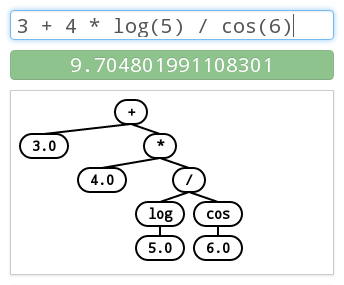
\includegraphics[scale=0.5]{figures/example-application.png}%
\end{center}%
\caption{The example application running on the Sunroof server.}%
\label{fig:example-application}
\end{figure}


The classical approach to develop an application like this would have 
been to write a server that provides a RESTful interface and replies 
through a JSON data structure. 
The client side of that application would have been written in JavaScript
directly.
This can be seen in \FigRef{fig:example-structure}.

\begin{figure}[h]%
%\vspace{-0.5cm}%
\begin{center}%
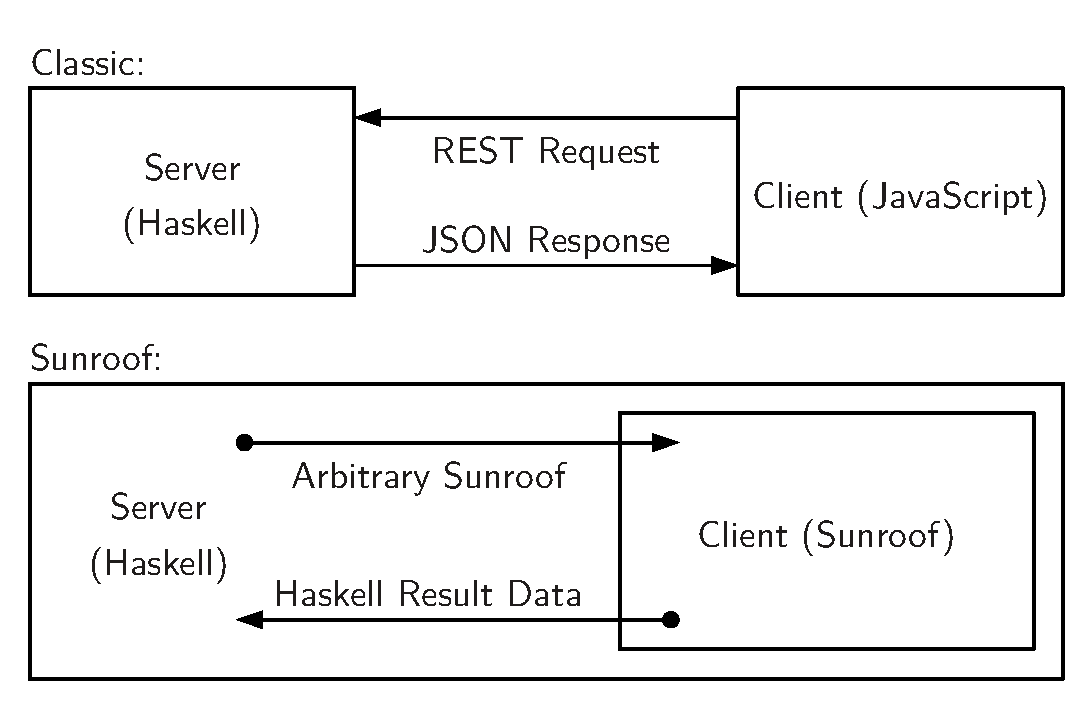
\includegraphics[scale=0.45,clip=true,trim=0.45cm 0.45cm 0.45cm 0.45cm]{figures/example-structure.pdf}%
\end{center}%
\caption{Classical structure and Sunroof structure of a web application.}%
\label{fig:example-structure}
\end{figure}


How does Sunroof improve or change this classical structure?
First of all, in Sunroof you write the client-side code together with
your server application within Haskell. In our example, all code 
for the server and client is in Haskell. The control logic 
for the client side is provided through the server.
This leads to a tight coupling between both sides. 
This also shows how Sunroof blurs the border between the server 
and client side. You are not restricted by an interface or language 
barrier. If you need the client to do something, you can just 
send arbitrary Sunroof code to execute in the client.
%
\TabRef{tab:example-statistics} contains a few statistics 
about the size of the code in each part of the client.

The client-server response loop shuffles new input to the server 
and executes the response in the client.
%
Data conversion is needed, because pure Haskell data types
cannot be handled in Sunroof and vice versa -- there still
exists this language barrier between JavaScript and Haskell. 
Data-structure definitions must be written
to allow conversion between two essentially equal data structures.
However, there is great potential in automatically 
generating this code using techniques such as template Haskell
\cite{Sheard:02:TemplateMetaProgrammingHaskell}.
Furthermore, this results in surprisingly readable JavaScript,
because these definitions are written to allow object fields
in the generated code to be used in the same way a native JavaScript
programer might.

The code for displaying the results is basically a 
transliteration of the JavaScript that you would write for this 
purpose.
The transliteration used here is not especially appealing. 
In the future, this code can be generated through higher-level 
libraries. Sunroof is intended to deliver a foundation for
this purpose.
The rest of our code to parse the arithmetic expression and calculate 
results is classical Haskell code. 

\begin{table}[t]
\begin{center}
\vspace{0.1in}
\begin{tabular}{l@{\quad}r@{\quad}r}
\hline\rule{0pt}{12pt}%
Part of Application & Lines of Code & Percentage \\[2pt]
\hline\rule{0pt}{12pt}%
Response loop & 25 & 6.5\% \\[2pt]
Data-structure Descriptions & 85 & 22.0\% \\[2pt]
Rendering & 190 & 49.5\% \\[2pt]
Parsing and interpretation & 85 & 22.0\% \\[2pt]
\hline
\end{tabular}
\end{center}
\caption{Lines of code needed for the example.}
\label{tab:example-statistics}
\vspace{-0.5cm}
\end{table} 

Overall, we were pleased with how our case study went.
It was possible to write an entire (small) application
in Sunroof, and use native JavaScript APIs, and have
the entire application compile to JavaScript. 

\section{Related Work}

There have been several attempts to translate Haskell to JavaScript.
Prominent ones are the compiler backends for 
UHC \cite{Stutterheim:12:ImprovingUHCJavaScriptBackend} and 
GHCJS \cite{project:ghcjs}. There are also projects like Fay \cite{project:fay} 
that compile subsets of Haskell to JavaScript or JMacro \cite{project:jmacro}
which use quasiquotation \cite{Mainland:07:QuasiquotingHaskell} to embed 
a custom-tailored language into Haskell code.
%
At the same time there are also projects like 
CoffeeScript \cite{project:coffeescript} or LiveScript \cite{project:livescript}
to build custom languages 
that are very similar to JavaScript but add convenient syntax and
support for missing features.

Our approach to cooperative concurrency through continuations in JavaScript has
has been used before 
\cite{Cooper:07:LinksWebProgrammingTiers,Predescu:02:CocoonContinuationBasedControlFlow}.
To our knowledge, creating a direct connection
between Haskell and JavaScript continuations has not been 
attempted before.

Deep embeddings of monads based on data structures have been used before
in Unimo \cite{Lin:06:Unimo} and Operational \cite{Apfelmus:10:Operational,Hackage:10:Operational}. 
The specific approach Sunroof takes 
by using GADTs has been discussed by 
Sculthorpe et al. \cite{Sculthorpe:13:ConstrainedMonads} 
in detail.

The Sunroof server does not have the aim to provide a full-featured 
web framework, as HAppS, Snap or Yesod do. It only provides 
the infrastructure to communicate with the currently calling website
through the Kansas comet \cite{project:kansas-comet} 
push mechanism \cite{pattern:push}. Although all of the
frameworks mentioned above would be able to implement this technique,
to our knowledge, none of them has yet.

To our knowledge, Sunroof is the only library that supports 
generation of JavaScript inside of Haskell using pure Haskell
in a type-safe manner. All other approaches discussed above
either require a separate compilation step or introduce new 
syntax inside of Haskell.
%
There also is an effort to generalize Active \cite{project:active}, a library for animations, and
implement a backend based on Sunroof \cite{project:sunroof-active}.

 
\section{Conclusion}

Sunroof took the key idea of monad reification and
successfully created the \JS-monad to describe computations
in JavaScript. This reification work was started by Farmer and
Gill \cite{Farmer:12:WebDSLs}, with the observation
of the possibility to reify a JS monad.
This paper documents the work since this initial prototype.
By stronger usage of types, and the concepts
of \Src{JSFunction} and \Src{JSContinuation}, there now is a 
stronger connection between
functions in the JavaScript and the Sunroof language space 
(\FigRef{fig:func-cont}). It is possible to go back and forth between 
both worlds. Combining both concepts, functions and the \JS-monad,
we were able to create a second implementation of the monad, this
time based on the direct translation of continuations from Haskell
to JavaScript. It enabled us to build a blocking threading model
on top of JavaScript that resembles the model already known from Haskell.
Based on this model and the provided abstraction over continuations,
we can use primitives like \Src{forkJS} or \Src{yield}.
Higher-level abstractions like \Src{JSMVar} and \Src{JSChan} are also
available. 

% 
\section{Conclusion}

We can see that Sunroof took the key idea of monad reification and
sucessfully created the \JS-monad to describe computations
in JavaScript. This work was mainly already done by Farmer and
Gill \cite{Farmer:12:WebDSLs} and has been streamlined during the 
further development of Sunroof. By adding the concept 
of \Src{JSFunction} and \Src{JSContinuation} there now is a connection between
functions as values in the JavaScript and the Sunroof language space 
(Figure \ref{fig:func-cont}). It is possible to go back and forth between 
both worlds. Combining both concepts, functions and the \JS-monad,
we were able to create a second implementation of the monad. This
time based on the direct translation of continuations from Haskell
to JavaScript. It enabled us to build a blocking threading model
on top of JavaScript that resembles the model already known from Haskell.
Based on this model and the provided abstraction over continuations
we can use synchronization primitives like \Src{forkJS} or \Src{yield}.
Higher level abstractions like \Src{JSMVar} and \Src{JSChan} are also
available. 


\section{Acknowledgments}

We want to thank Conal Elliott for his support in adapting 
the Boolean package \cite{project:boolean} and helping us to
extend it with support for deeply embedded numbers.

%
% ---- Bibliography ----
%
\bibliographystyle{splncs03}
\bibliography{sunroof}
\vspace{-0.5cm} % THIS SAVED MY LIFE

\end{document}
